
\begin{SCfigure*}
	\centering
	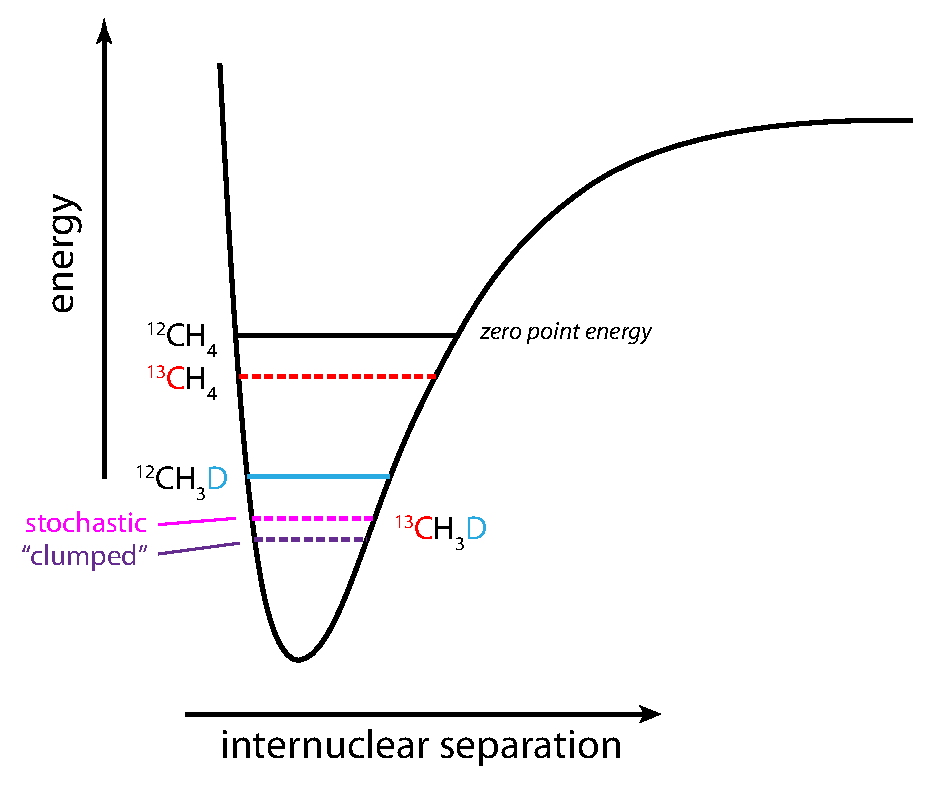
\includegraphics[width=0.55\textwidth]{figures/Fig1.4.pdf}
	\captionsetup{format=myformat}	% hrule beneath caption
	\caption[Statistical mechanical origin of preferential heavy-isotope clumping]{Zero-point energy lowering and the origin of non-stochastic clumped isotopologue composition
		at equilibrium.  The zero-point energy (the energy of the ground state, the quantum state with the lowest possible energy) of a molecule of methane is lowered upon substitution of heavy isotopes.  The amount by which the zero-point energy is lowered upon double-isotope substitution (e.g., \ce{^{12}CH4} to \ce{^{13}CH3D}) is slightly greater than the sum of the effects of substituting only one heavy isotope (to make \ce{^{13}CH4} and \ce{^{12}CH3D}).  This deviation from the ``rule of the geometric mean'' \parencite{Bigeleisen_1955_JCP} is particularly pronounced at lower temperatures, and is the origin of the preferential clumping at equilibrium shown in \autoref{fig:1:3}.  For a detailed treatment, readers are referred to \textcite{Eiler_2007_EPSL}.}
	\label{fig:1:4}
\end{SCfigure*}